The theoretical context has been set, now the study of a Neural Network as an improvement over the Random Decision Forest will be presented.

\section{Tools used}

This study follows on from years of software development inside the KM3NeT collaboration, and beyond. The data analysis in this experiment is done using the framework ROOT, which see a lot of use in particle physics, and to which new libraries proper to the collaboration are added. The neural network has been built using a ROOT package named Toolkit for Multivariate Data Analysis \citep{2007physics...3039H}, or TMVA.

The Letter of Intent shows the use of a RDF with 101 trees using close to two hundred variables reconstructed from the raw data of the detector. The neural network built is compared to this RDF.

As in the Letter of Intent \citep{Adrian-Martinez:2016fdl}, or LoI, two broad classes have been defined: "track-like" neutrino events, and "shower-like" neutrino events. The former are those induced by charged-current muon neutrino (and antineutrino) interactions, and appear in the detector as a long track. The latter are induced by all neutral current neutrino (and antineutrino) interactions, as well as charged current electron neutrino (and antineutrino) interactions, and appear in the detector as a point-like event. The two final classes, once classified by the neural network, are named "seen as track-like" and "seen as shower-like".

The dataset used in this study come in the form of a tree of 4,786,617 simulated events (Monte Carlo simulation): 1,457,943 track-like events, and 3,328,674 shower-like events, every events in this tree sharing the same data structure. Half of that is used during the training of the neural networks, and their performance are evaluated on the other half, constituting the test sample.

Thirty variables are fed to the neural network, such as the reconstructed energy, the number of PMTs hit, the total number of photons received by these PMTs, the spread of the x, y and z-distributions of hit DOMs, and many other variables built from the raw data recorded by the virtual detector during the simulation. The pool have been chosen based on the previous RDF classification, by selecting the best performing variables, and after many tries of different combinations, the best performing network has been chosen.

To compare the Neural Network and the RDF, quantities able to evaluate the classification must be defined.

\section{Useful Plots: Example of the RDF}

Two quantities have been compared: the efficiencies of the classifications and the purities of the resulting classes.

\subsection{Standard PID plot}

\qquad The LoI \citep{Adrian-Martinez:2016fdl} introduced a standard plot to evaluate the performance of the RDF classification. Shown in Fig. \ref{fig:JYVHJ}, this plot represents, as functions of the true energy of the neutrino (known because the dataset is the result of a simulation), the fraction of events identified as track-like for each class. This fraction for the track-like class is an efficiency, while for the shower-like events, the efficiency is equal to one minus the plotted fraction. This result is obtained by choosing a cut on the classifier output at 0.5.

\begin{figure}[h!]
    \centering
    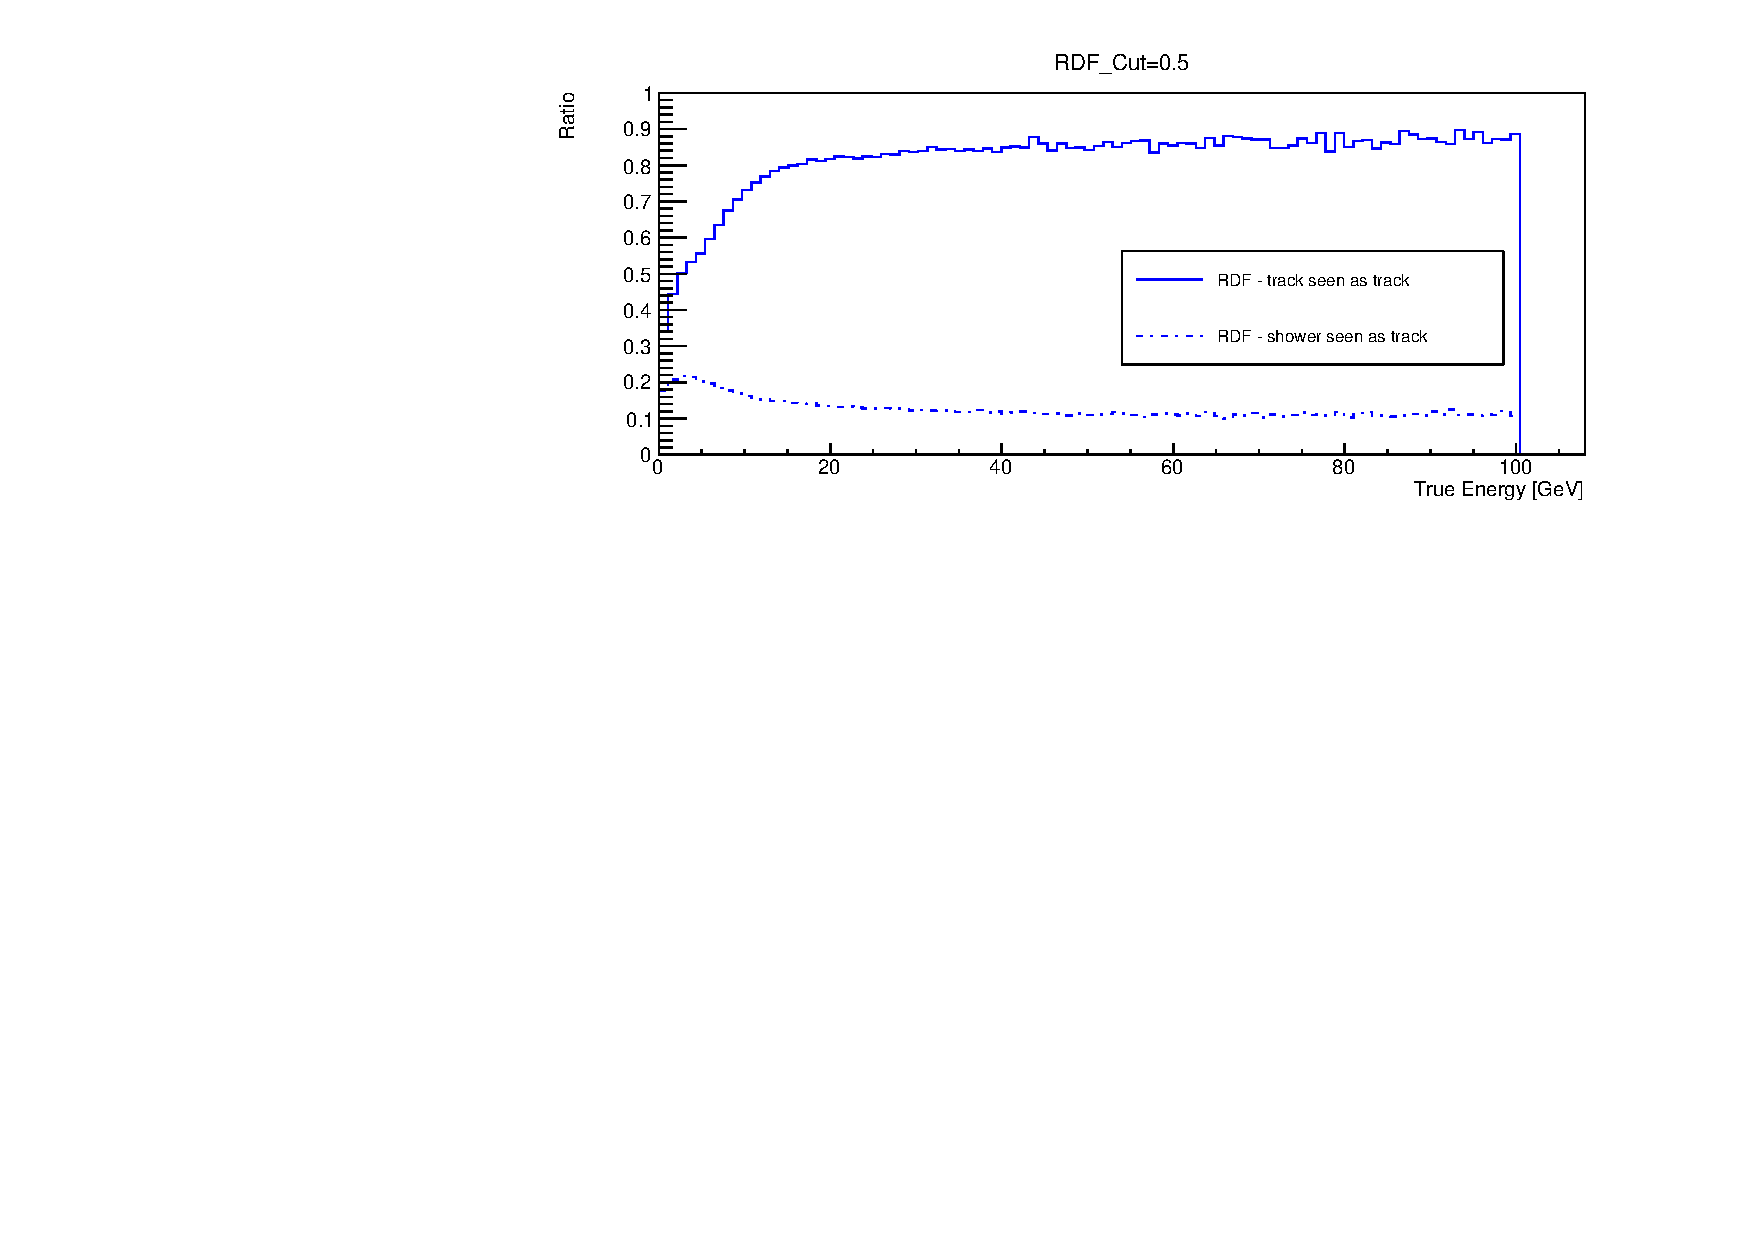
\includegraphics[width=0.9\textwidth]{fig/PID_Efficiency_RDF_CUT_0_5_E_cut_100.pdf}
    \caption{Ratio of track-like events (full line) and shower-like events (dotted line) seen as track, as a function of the true energy --- 0--100 GeV range --- cut = 0.5 --- RDF}
    \label{fig:JYVHJ}
\end{figure}

This plot can be divided into two parts. One above 20 GeV, where the two fractions are constant, and where the classifier performs well: close to 90\% of the track-like events are classified correctly, and no more than 10\% of the shower-like events are incorrectly classified. In the other part, below 20 GeV, the classification gets significantly worse: the fraction of track-like events correctly identified decreases abruptly, and the fraction of incorrectly classified shower-like events slowly increases. Though unfortunate, this trend is not surprising as, the lower the energy of a muon neutrino, the lower the energy of the muon created through a CC muon-neutrino event, and the lower the length of the muon track in the detector. Thus low energy CC muon neutrino events tend to look closer to shower-like events.

\subsection{Purity plot}

\qquad When comparing the results of two different trainings, it is sometimes difficult to tell which training led to a better result, for example when the fraction of events classified as track-like decreases for both classes. Another quantity can be defined for each of the two final classes, "seen as track-like" and "seen as shower-like": the purity, like in Eq. \refeq{EIOZ}, measuring the ratio of correctly classified events in regards to the total number of events classified, in one category.

\begin{equation}
    \left\{
    	\begin{array}{ll}
    		Purity(\text{track-like})=\frac{\text{\large N(track-like\;seen\;as\;track)}}{\text{\large N(track-like\;seen\;as\;track) + N(shower-like\;seen\;as\;track)}} \\[10pt]
		    Purity(\text{shower-like})=\frac{\text{\large N(shower-like\;seen\;as\;shower}}{\text{\large N(track-like\;seen\;as\;shower) + N(shower-like\;seen\;as\;shower)}}
    	\end{array}
   	\right.
    \label{EIOZ}
\end{equation}
where N(class) is the number of events in the class considered.

The purity of each class for the RDF is plotted in Fig. \ref{fig:KJINDE}, again as a function of the true energy of the neutrino, and for a cut on the classifier output at 0.5.

\begin{figure}[h!]
    \centering
    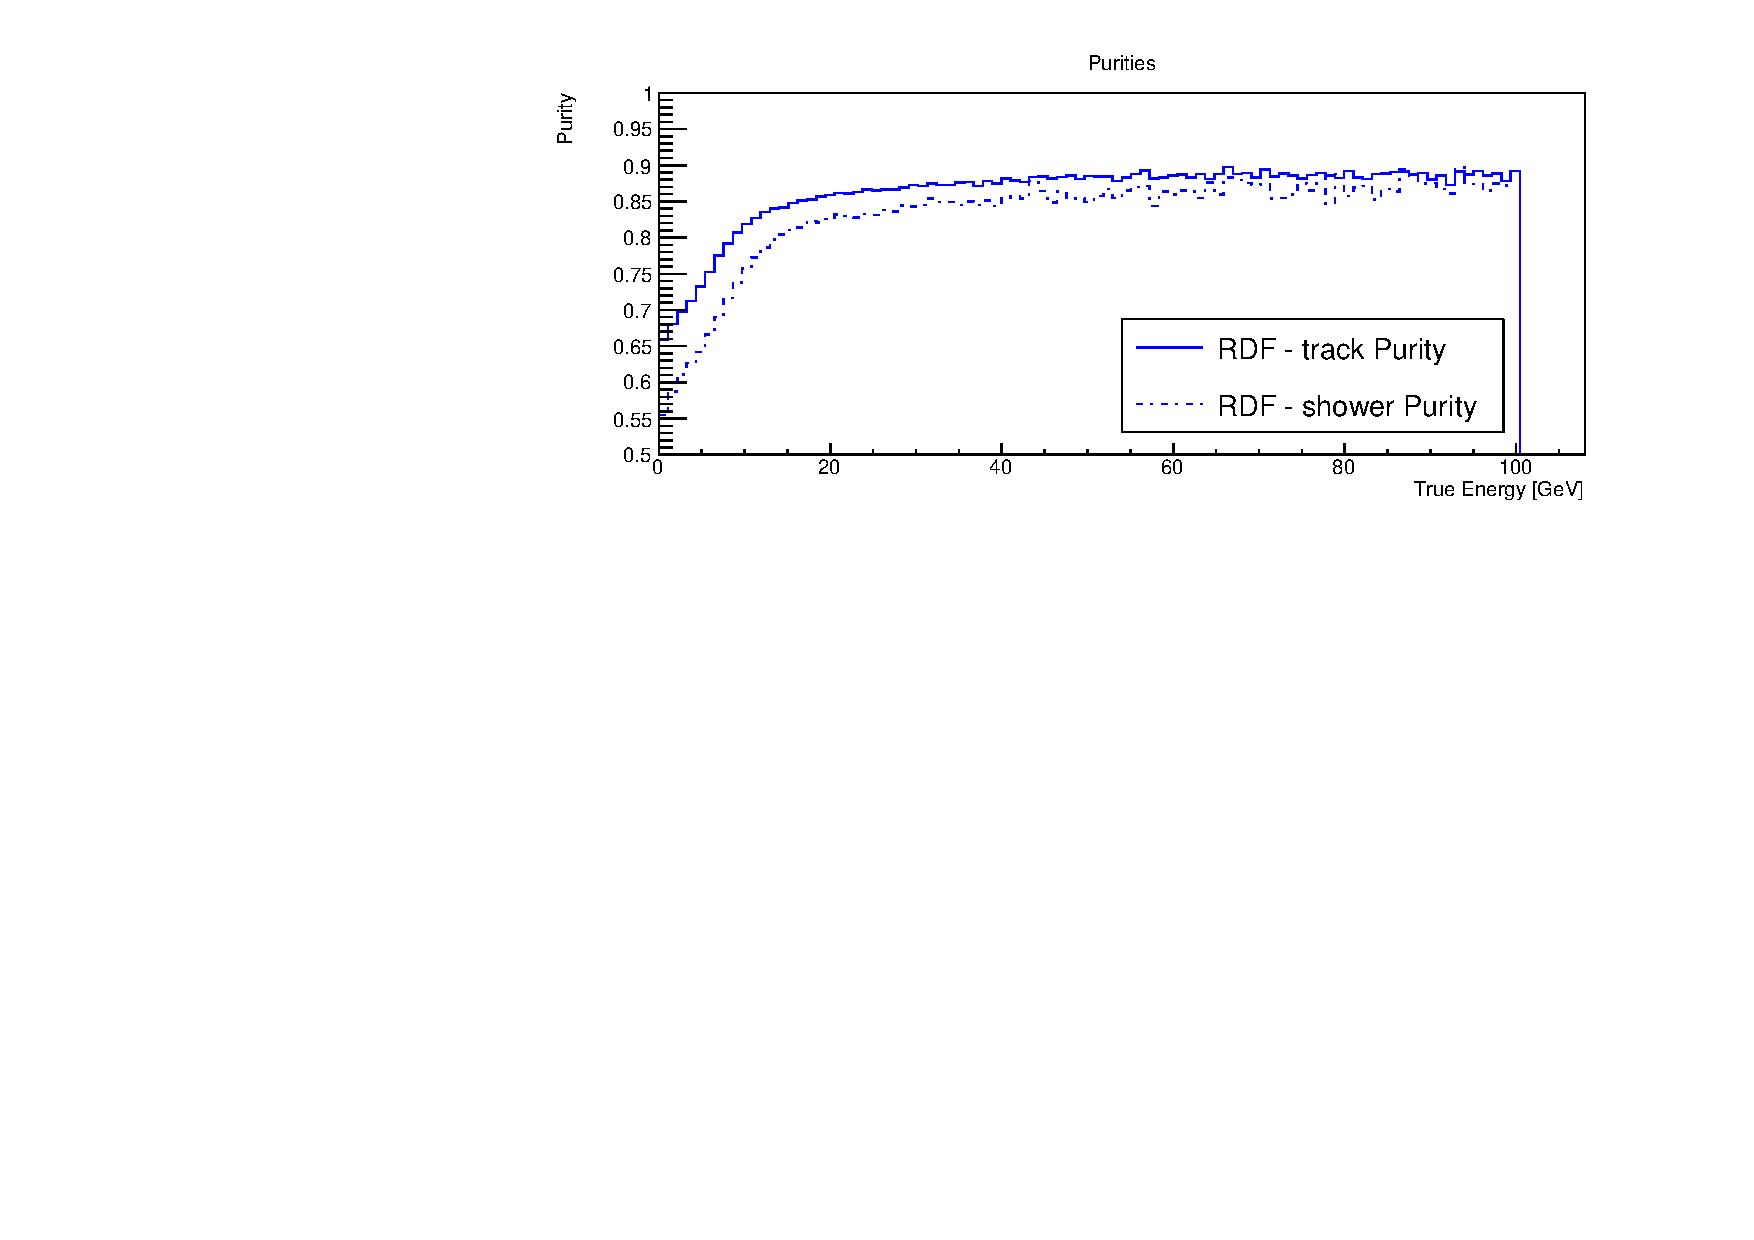
\includegraphics[width=0.9\textwidth]{fig/PID_Purity_RDF_CUT_0_5_E_cut_100.pdf}
    \caption{Purities of the track-like (full lines) and shower-like (dotted lines) classes, as a function of the true energy  --- 0--100 GeV range --- cut = 0.5 --- RDF}
    \label{fig:KJINDE}
\end{figure}

The same two parts can be seen here, with purities relatively constant above 20 GeV, and a drop at low energy, with the seen as shower-like class dropping as low as 55\% purity. Because track-like events tend to be identified as showers at low energies while the proportion of badly classified shower-like events remains rather constant, the purity of the seen as shower class remains lower than the purity of the other class.

The results presented in this section correspond to a cut value on the classifier output of 0.5. What is the influence of the cut value on these efficiencies and on those purities?

\section{Influence of the cut on the classifier output}

\paragraph{} As it has been said in section 1.2.2 the value of the cut will greatly affect the result of the classification. In this study we decided to apply only one cut, and not to discard any event. In Fig. \ref{fig:JHYD}, we can see the effect of the cut on the standard PID plot for the RDF, for the track-like events on the top plot, and the shower-like events on the bottom plot. As the value of the cut increases, both ratio decrease as we can see in Fig. \ref{fig:ABHD}, where the classifier output distribution of the RDF is represented with the cut positioned at 0.5.. As we shift the cut towards 1, we simply ask for events to have more characteristic patterns for the neural network to classify them as track-like ($\hat{y_a}=1$). But as this one class thus increases its purity, the other one's purity gets worse.

\begin{figure}[!h]
    \centering
    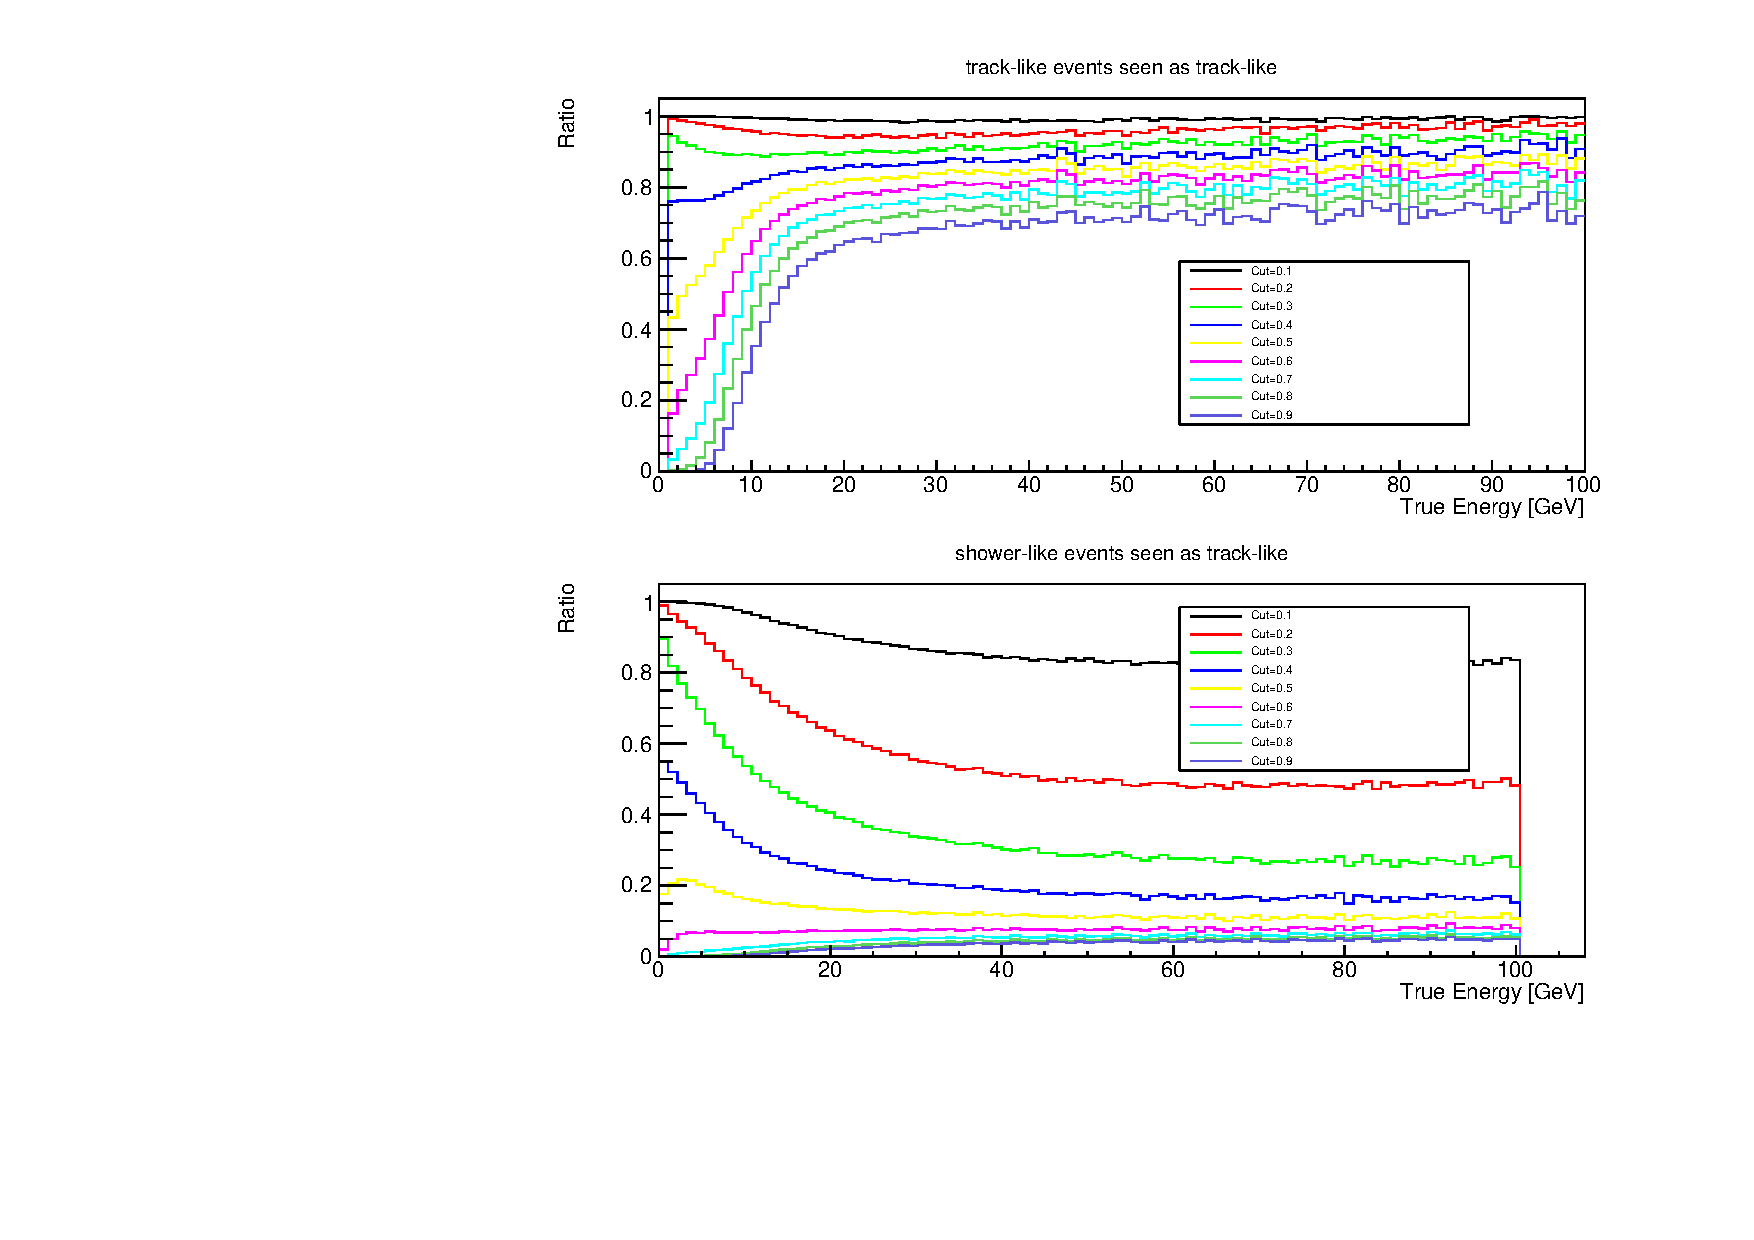
\includegraphics[width=0.9\textwidth]{fig/Cuts_comparison.pdf}
    \caption{Ratio of track-like events (top) and shower-like events (bottom) seen as track, as a function of the true energy, for various values of the classifier cut --- 0--100 GeV range --- RDF}
    \label{fig:JHYD}
\end{figure}

\begin{figure}[!h]
    \centering
    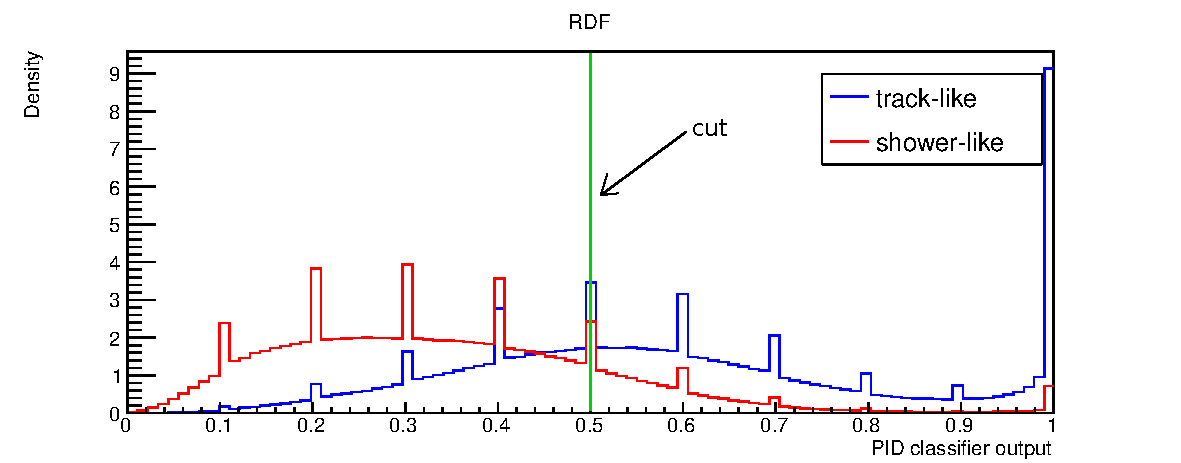
\includegraphics[width=0.9\textwidth]{fig/PID_Classifier_RDF_E_cut_100.pdf}
    \caption{Distributions of the classifier output of the test sample classified by the RDF, for the shower-like events (red) and track-like events (blue). Each distribution is normalised to the total number of events considered. The green line represents the position of the cut.}
    \label{fig:ABHD}
\end{figure}

\paragraph{}
The usual values adopted for the cut remain around 0.5. Such values keep a balance between the purities of the two classes, and the efficiency of the classification for both class. This is no different for the neural network built.

\newpage
\section{Our neural network}

\paragraph{}
The RDF has been trained using all the reconstruction variables available: a number close to two hundred. The neural network, as we said in section 2.1, is only fed thirty variables. The performance of the neural network is compared to the one of the RDF: in Fig. \ref{fig:INLDN} the standard PID plots, and in Fig. \ref{fig:OIDLMRU} the purities of the track-like and and of the shower-like classes. In the two figures, the neural network's performance is shown in red, and the RDF's in blue. The neural network's cut value of 0.6 is chosen so that it matches the RDF performance.

At high energy, the results are similar. The efficiencies are close, the RDF having a better efficiency for the track-like channel while the neural network does better in the shower-like channel. The purities also cannot be used to chose a better classification: the neural network has a better track purity and a worse shower purity, while the RDF sits in the middle for both. However, at low energy the neural network seems to be ahead.

\begin{figure}[!h]
    \centering
    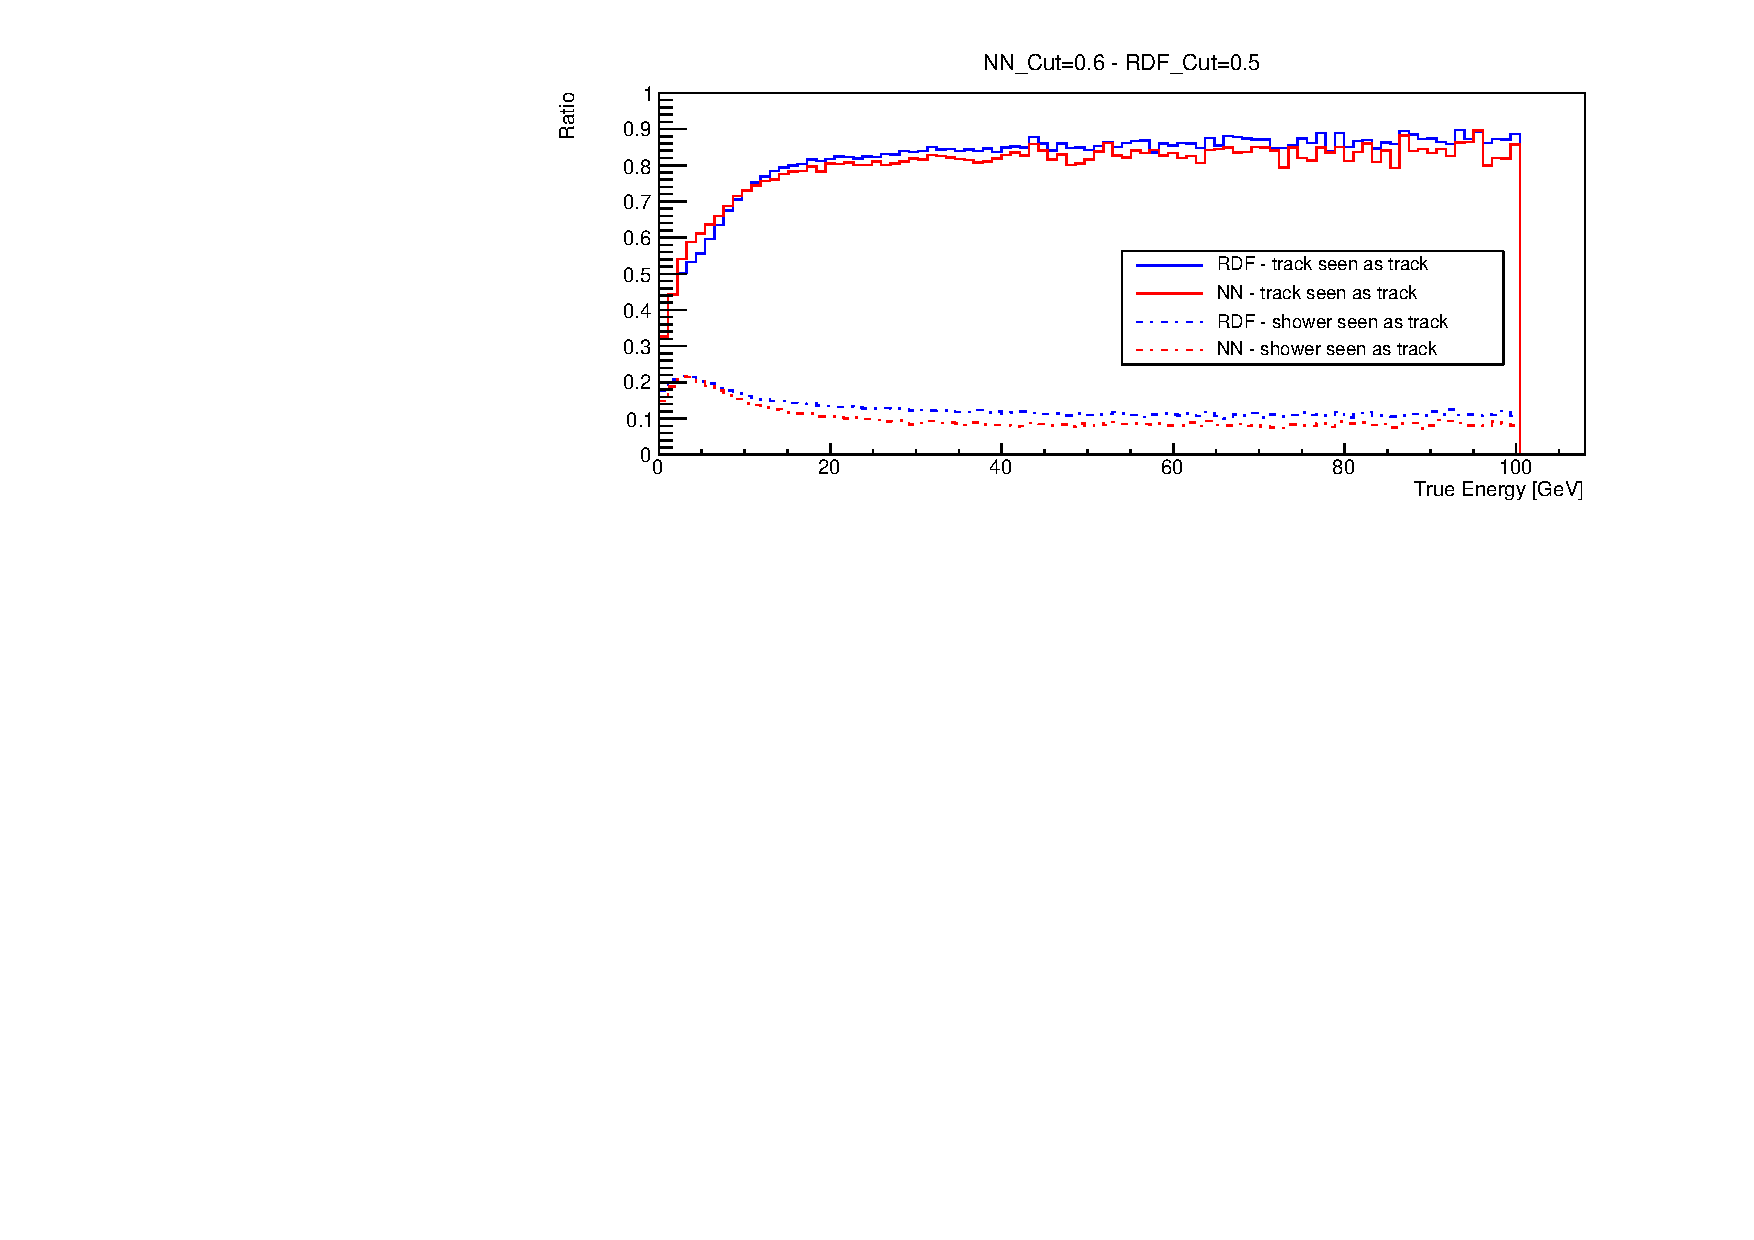
\includegraphics[width=0.9\textwidth]{fig/PID_Efficiency_RDF_CUT_0_5_VS_NN_CUT_0_6_E_cut_100.pdf}
    \caption{Ratio of track-like events (full lines) and shower-like events (dotted lines) seen as track, as a function of the true energy, for the NN (red) and the RDF (blue)  --- 0--100 GeV range --- RDF cut = 0.5 --- NN cut = 0.6}
    \label{fig:INLDN}
\end{figure}

\begin{figure}[!h]
    \centering
    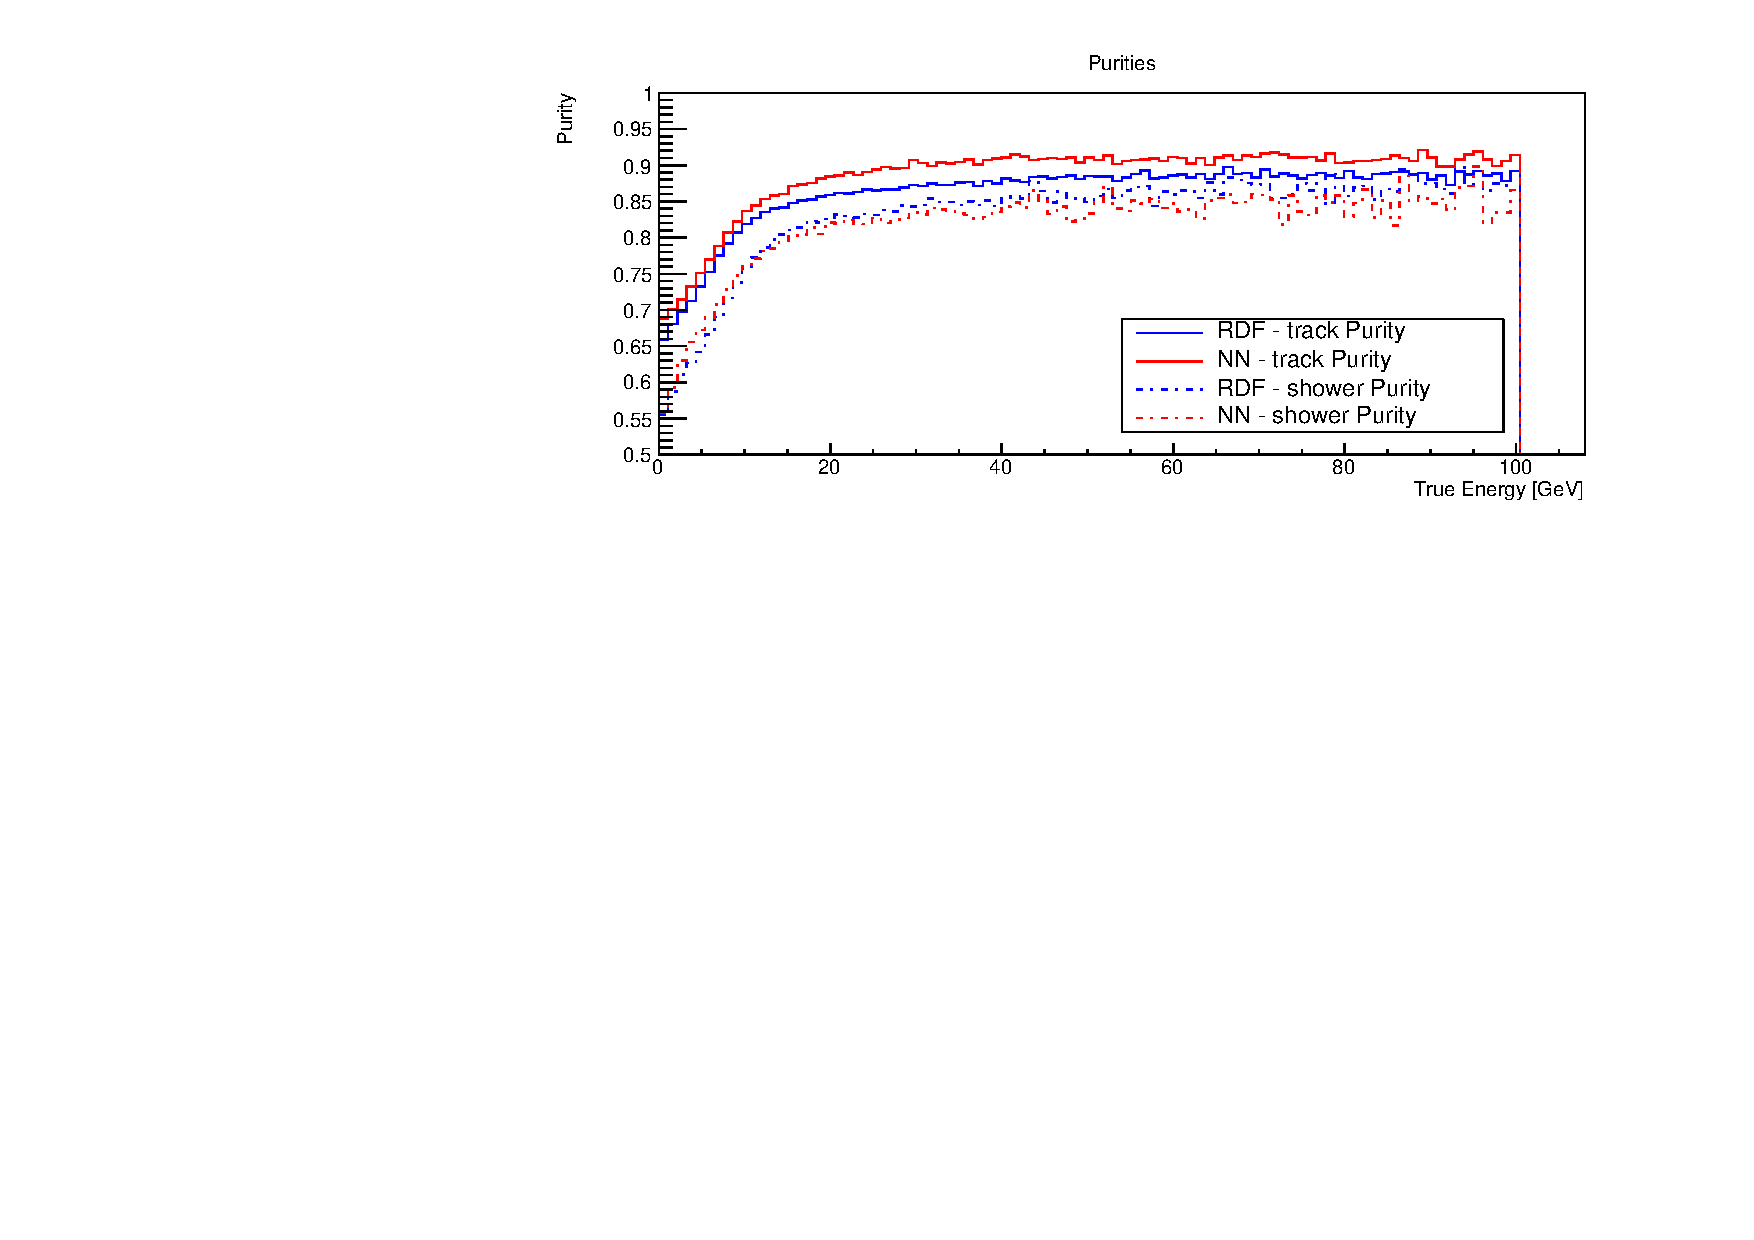
\includegraphics[width=0.9\textwidth]{fig/PID_Purity_RDF_CUT_0_5_VS_NN_CUT_0_6_E_cut_100.pdf}
    \caption{Purities of the track-like (full lines) and shower-like (dotted lines) classes, as a function of the true energy, for the NN (red) and the RDF (blue)  --- 0--100 GeV range --- RDF cut = 0.5 --- NN cut = 0.6}
    \label{fig:OIDLMRU}
\end{figure}

Indeed, a zoom onto the low-energy range shows a clear improvement using the neural network. In Fig. \ref{fig:EUFBKBF}, the standard PID plot is shown for energies in the range 1--20 GeV, witht the same colour code as previously. The neural network has a lower ratio of incorrectly classified shower-like events in the whole range, and the ratio of correctly classified track-like events stays close to the one of the RDF for most of the energy range, except around 4 GeV where the neural network see the best improvement. The purity plot in Fig. \ref{fig:SLKNPE} shows the neural network ahead in the whole 1--20 GeV energy range, in terms of purity, which amply compensates for the slight loss of efficiency. As we are interested in the 1--10 GeV range, this is an interesting result.

\begin{figure}[!h]
    \centering
    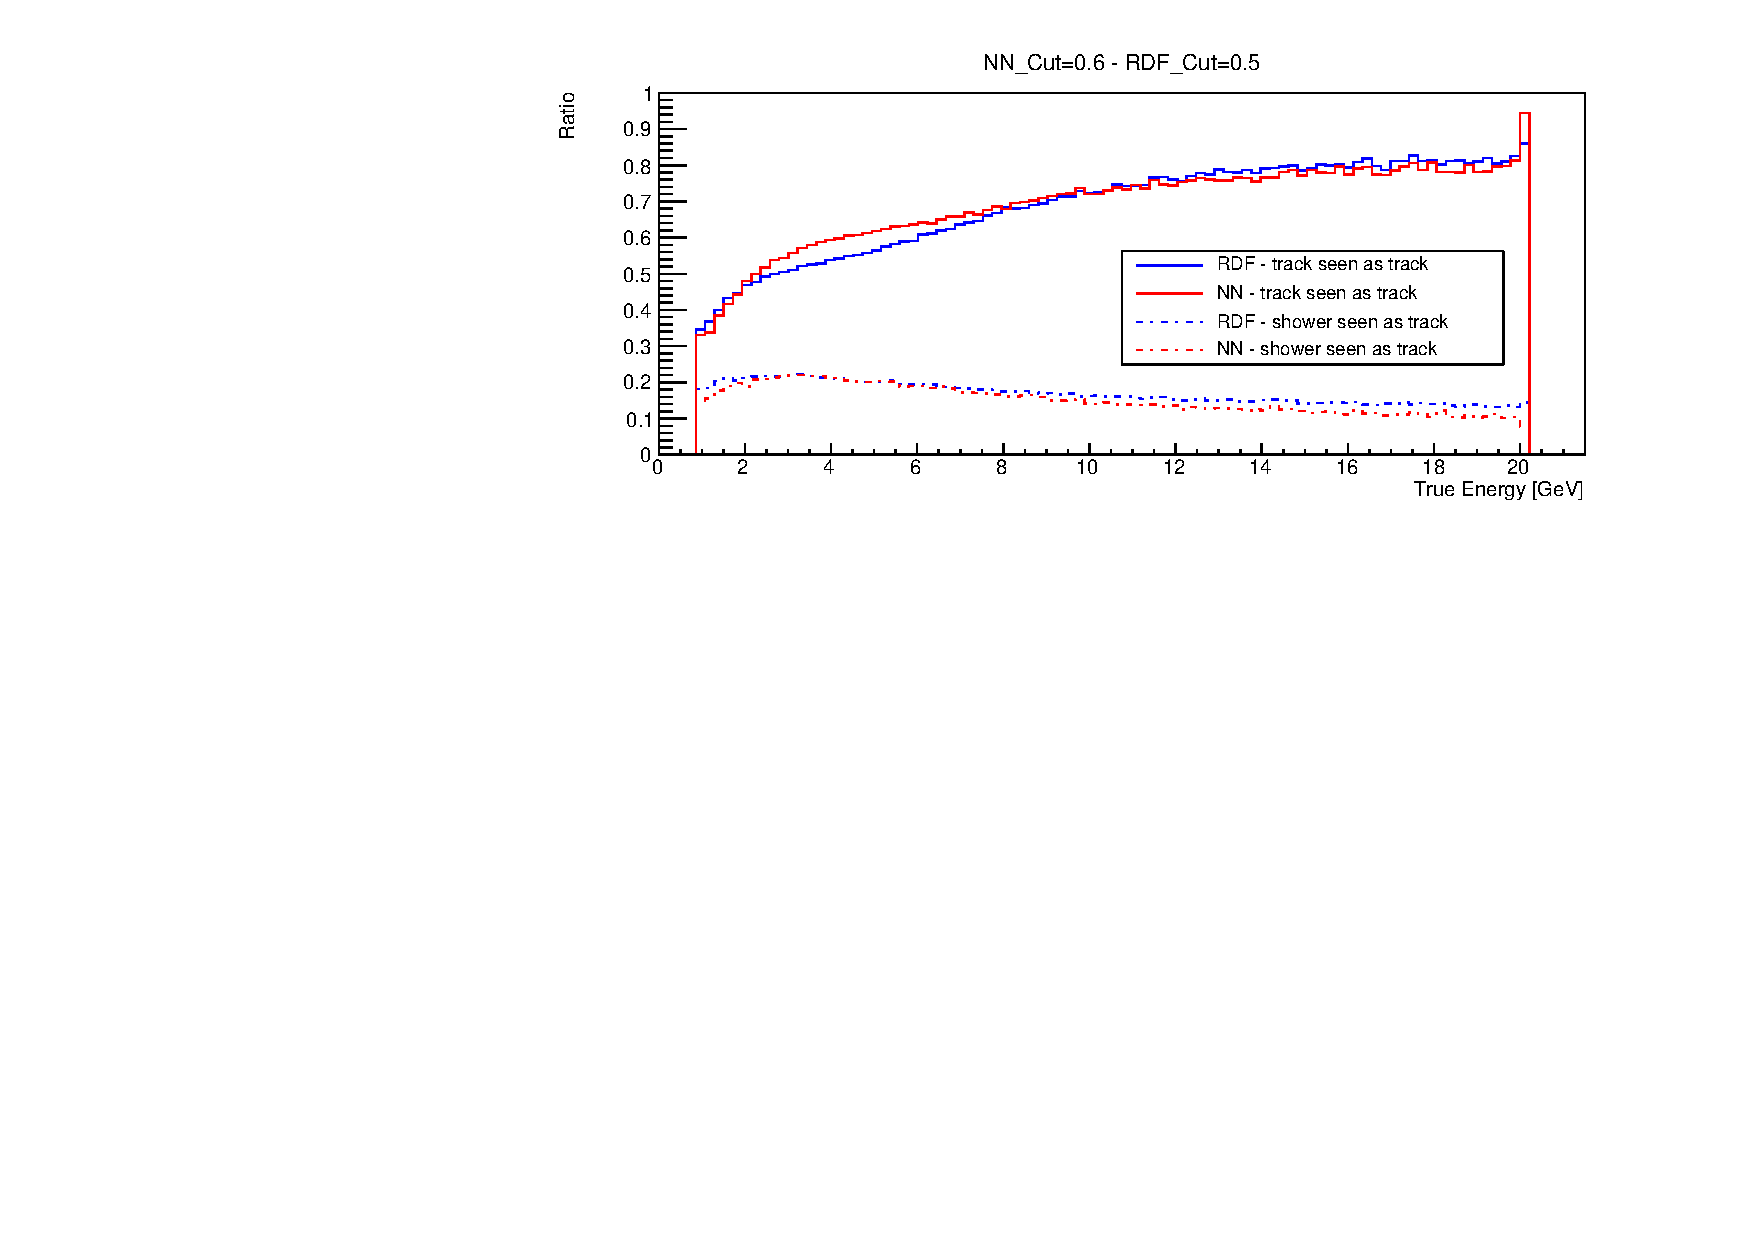
\includegraphics[width=0.9\textwidth]{fig/PID_Efficiency_RDF_CUT_0_5_VS_NN_CUT_0_6_E_cut_20.pdf}
    \caption{Ratio of track-like events (full lines) and shower-like events (dotted lines) seen as track, as a function of the true energy, for the NN (red) and the RDF (blue)  --- 0--20 GeV range --- RDF cut = 0.5 --- NN cut = 0.6}
    \label{fig:EUFBKBF}
\end{figure}

\begin{figure}[!h]
    \centering
    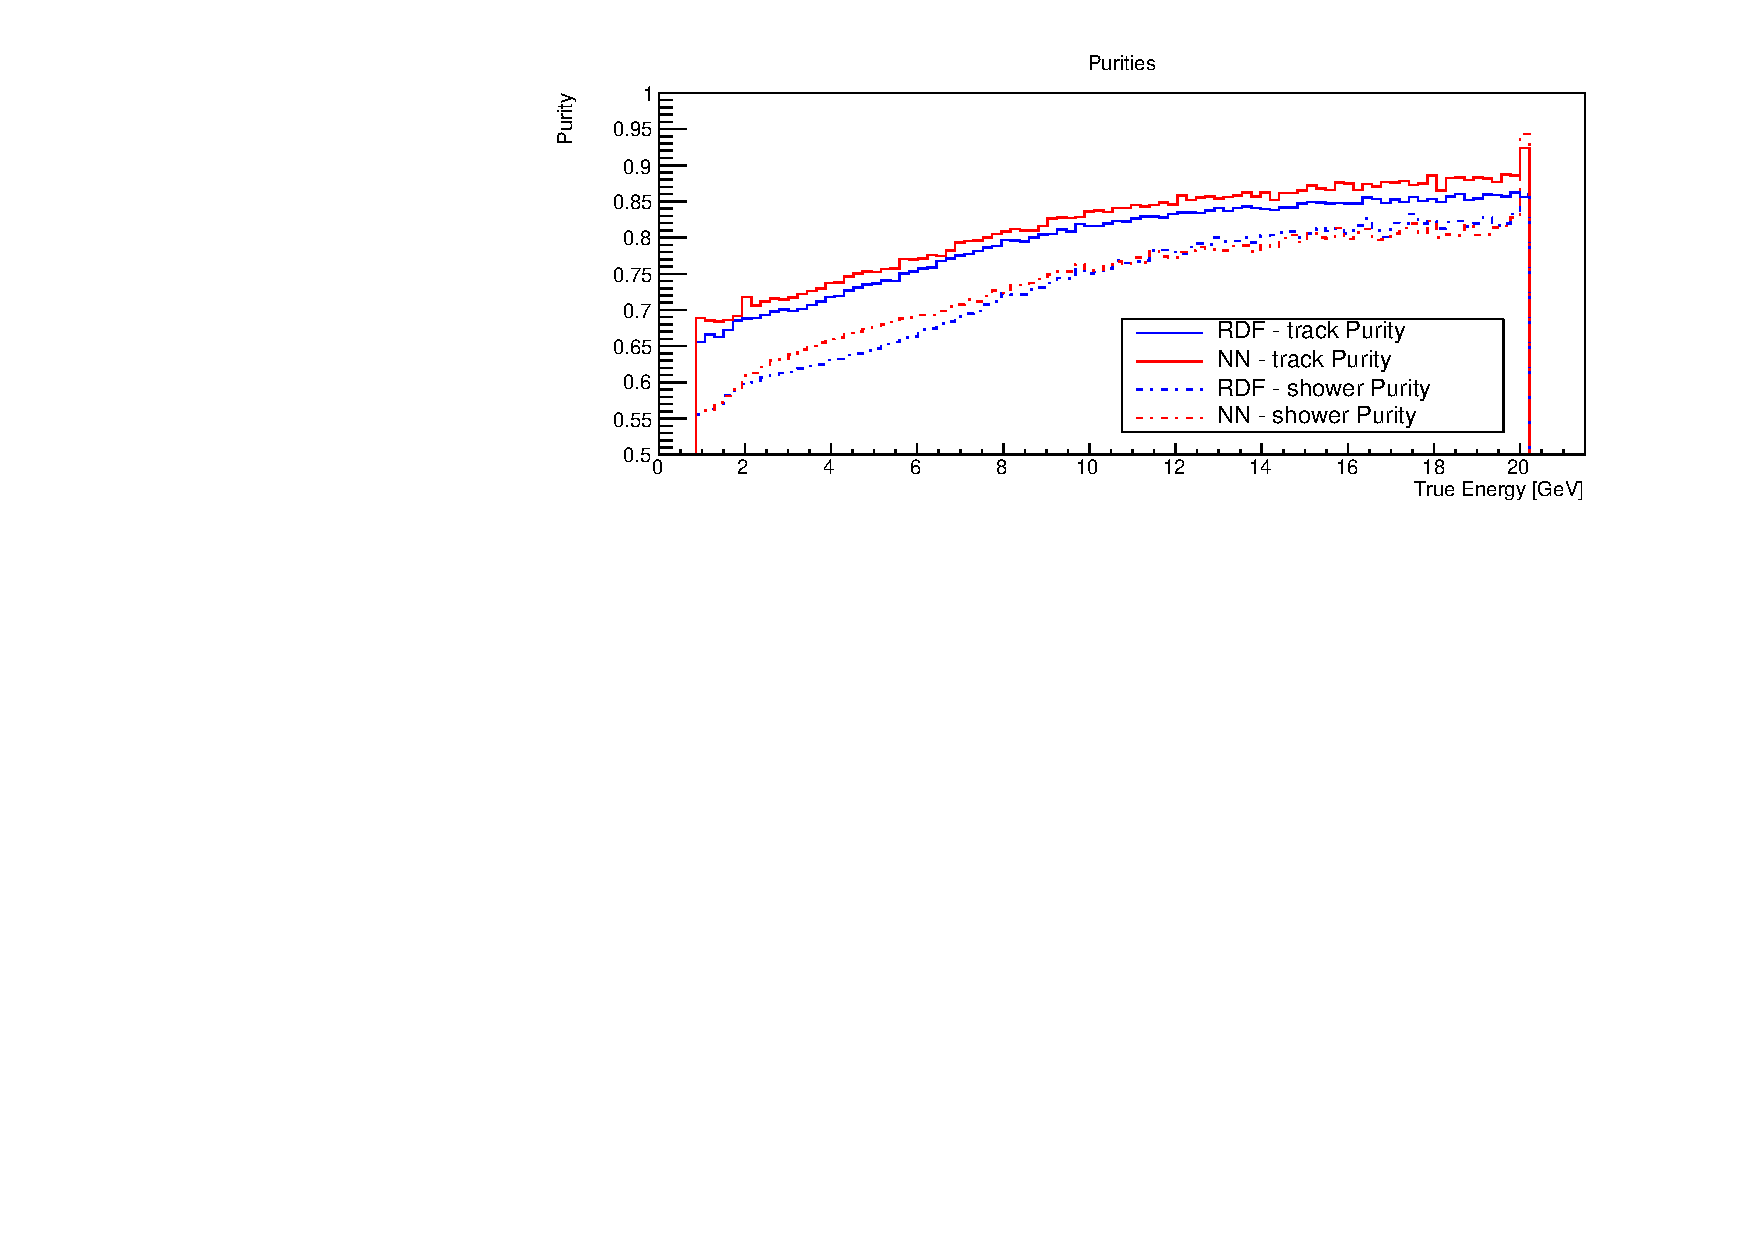
\includegraphics[width=0.9\textwidth]{fig/PID_Purity_RDF_CUT_0_5_VS_NN_CUT_0_6_E_cut_20.pdf}
    \caption{Purities of the track-like (full lines) and shower-like (dotted lines) classes, as a function of the true energy, for the NN (red) and the RDF (blue)  --- 0--20 GeV range --- RDF cut = 0.5 --- NN cut = 0.6}
    \label{fig:SLKNPE}
\end{figure}

This neural network validates two of the objectives set at the beginning of this study. First its classification at low energies outperforms the one of the Random Decision Forest, and although the absolute gain shown in the efficiency plots is slight, the relative improvement as seen in the purity plots is not negligible. Besides that, this neural network only uses thirty variables, much less than the close-to-two-hundred variables needed for the Random Decision Forest.

\chapter*{Conclusion}
\addcontentsline{toc}{chapter}{Conclusion}

The objective of this work was to improve the particle identification at the energy-range 1--10 GeV, and to reduce the number of variables used in the classification. The first part of this report presented the NMH problem and how KM3NeT/ORCA plans to solve it, and introduced the tools necessary to the PID. The second part detailed the construction of the neural network used in this work as well as the quantities that would then be used to compare the performance of this same neural network with the one of the RDF. The conclusion is that both objectives have been reached, as the neural network both outperforms the Random Decision Forest and uses less variables than it.

There is still a lot of room for improvement: obviously all the combinations of variables have not been studied, and selecting variables solely on their individual performance, as we did in this study, does leave a lot of good possible candidates out: indeed, a neural network extract the information from the whole multi-dimensional space we feed it, and can thus see correlations between variables that can help for the classification. However, testing all the possible pools of variables would necessitate a lot of computing power, as just one set of 30 variables takes around 24 hours for the neural network to train on the machines used during this work. Another approach should be found.


